\section{Data Modelling}

\begin{frame}{Data Modelling}

  \begin{itemize}
    \item Data looks like a skewed bell curved
    \item Modelled using Normal Distribution
  \end{itemize}
  
\end{frame}


\subsection{Box-Cox transformation}

\begin{frame}{Box-Cox Transformation}

  Used box-cox transformation to reduce skewness.

  \[
    \text{Box-Cox}(x_i; \lambda) =
    \begin{cases}
    \frac{1}{\lambda} (x_i ^ \lambda - 1) & \lambda \ne 0 \\
    \ln x_i & \lambda = 0
    \end{cases}
  \]

  \begin{figure}
    \centering
    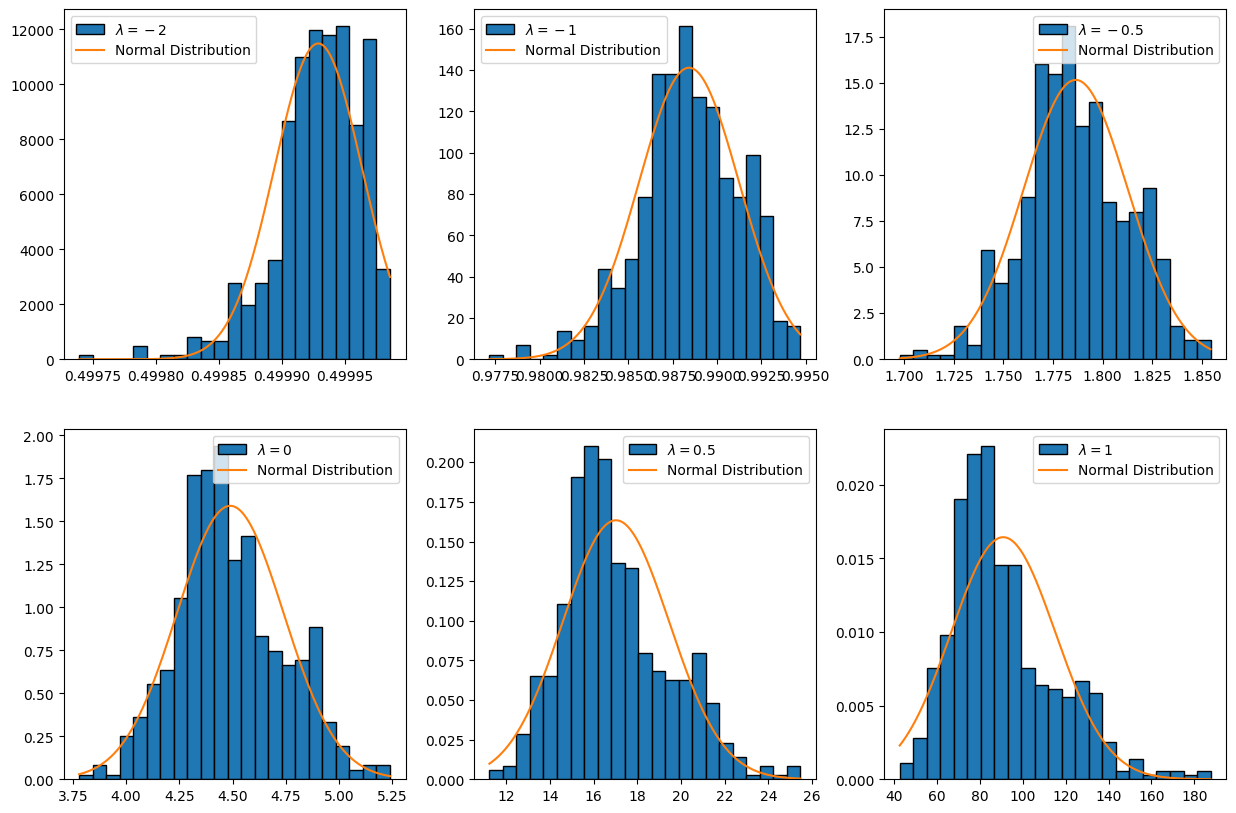
\includegraphics[width=0.7\linewidth]{../Report/images/transforms.png}
    \caption{Transformation with different $\lambda$}
  \end{figure}
  
\end{frame}


\subsection{Q-Q plots}

\begin{frame}{Q-Q plots}

  Used Q-Q (Quantile-Quantile) plots to visualize how well our transformation fits the normal distribution.

  \vspace{0.25in}
  \begin{figure}
    \centering
    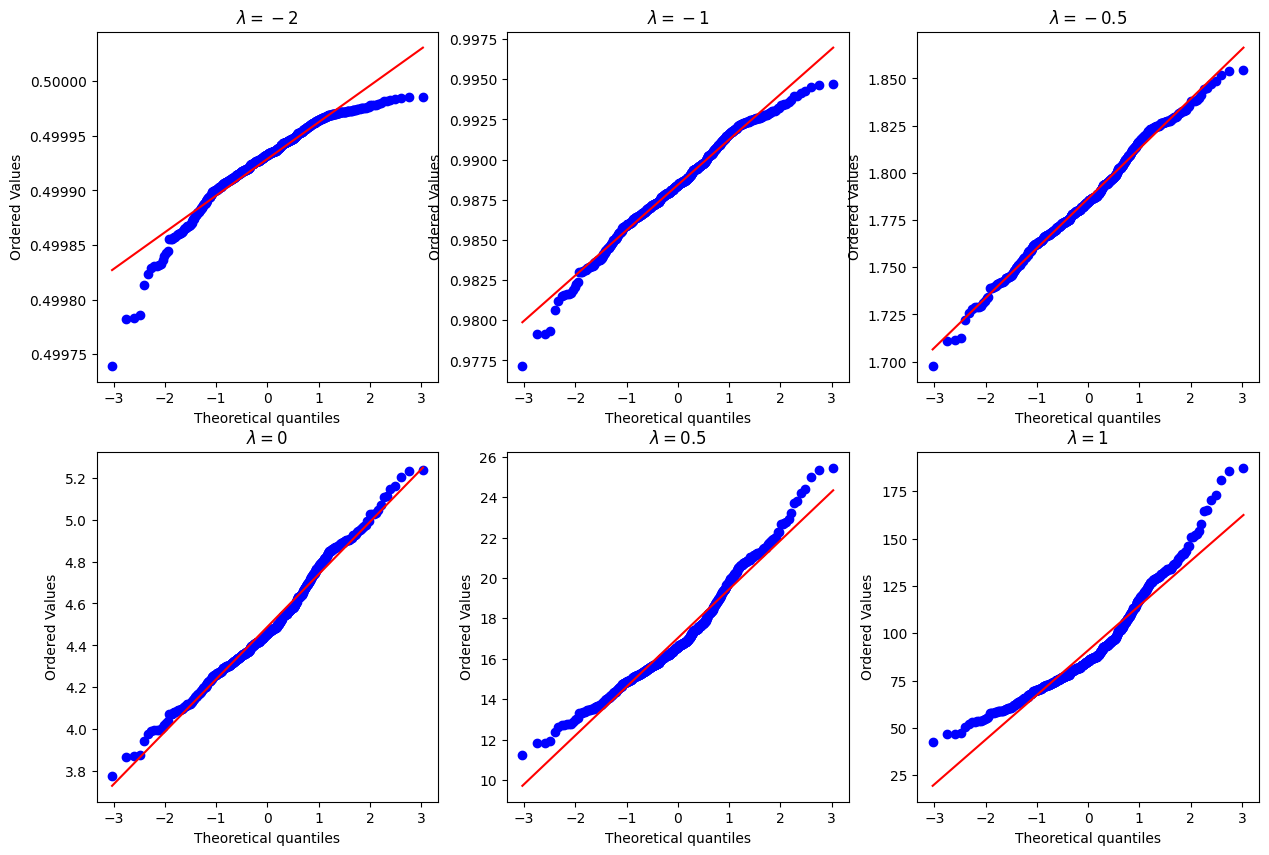
\includegraphics[width=0.8\linewidth]{../Report/images/q-q.png}
    \caption{Q-Q Plot with different $\lambda$}
  \end{figure}

\end{frame}


\subsection{Pearson's correlation}

\begin{frame}{Finding Optimal $\lambda$}

  The normality of the transformation is calculated as Pearson's correlation coefficient between the theoretical quantiles and the observed quantiles.

  \[ r(x, y) = \frac{\overline{xy} - \bar{x} \cdot \bar{y}}{\sigma_x \cdot \sigma_y} \]

  \vspace{0.25in}
  \begin{figure}
    \centering
    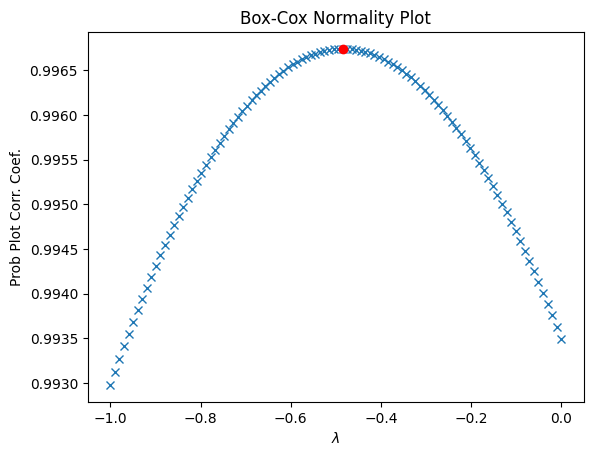
\includegraphics[width=0.6\linewidth]{../Report/images/normality.png}
    \caption{Optimal $\lambda$}
  \end{figure}
  
\end{frame}

\begin{frame}{Finding Optimal $\lambda$}

  \begin{figure}
    \centering
    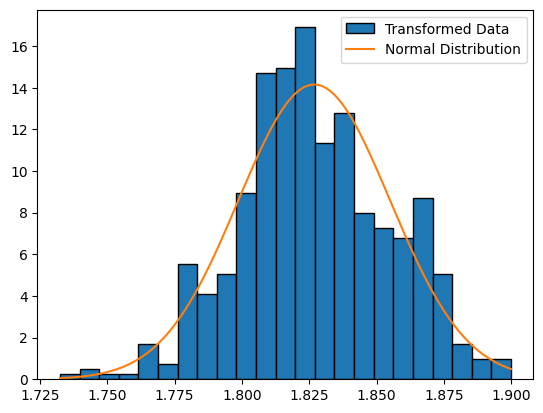
\includegraphics[width=0.8\linewidth]{../Report/images/optimal-hist.png}
    \caption{Histogram of Data with Optimal $\lambda$}
  \end{figure}
  
\end{frame}
